% Template for Cogsci submission with R Markdown

% Stuff changed from original Markdown PLOS Template
\documentclass[10pt, letterpaper]{article}

\usepackage{cogsci}
\usepackage{pslatex}
\usepackage{float}
\usepackage{caption}

% amsmath package, useful for mathematical formulas
\usepackage{amsmath}

% amssymb package, useful for mathematical symbols
\usepackage{amssymb}

% hyperref package, useful for hyperlinks
\usepackage{hyperref}

% graphicx package, useful for including eps and pdf graphics
% include graphics with the command \includegraphics
\usepackage{graphicx}

% Sweave(-like)
\usepackage{fancyvrb}
\DefineVerbatimEnvironment{Sinput}{Verbatim}{fontshape=sl}
\DefineVerbatimEnvironment{Soutput}{Verbatim}{}
\DefineVerbatimEnvironment{Scode}{Verbatim}{fontshape=sl}
\newenvironment{Schunk}{}{}
\DefineVerbatimEnvironment{Code}{Verbatim}{}
\DefineVerbatimEnvironment{CodeInput}{Verbatim}{fontshape=sl}
\DefineVerbatimEnvironment{CodeOutput}{Verbatim}{}
\newenvironment{CodeChunk}{}{}

% cite package, to clean up citations in the main text. Do not remove.
\usepackage{cite}

\usepackage{color}

% Use doublespacing - comment out for single spacing
%\usepackage{setspace}
%\doublespacing


% % Text layout
% \topmargin 0.0cm
% \oddsidemargin 0.5cm
% \evensidemargin 0.5cm
% \textwidth 16cm
% \textheight 21cm

\title{Determining the alternatives for scalar implicature}


\author{{\large \bf Benjamin Peloquin} \\ \texttt{bpeloqui@stanford.edu} \\ Department of Psychology \\ Stanford University \And {\large \bf Michael C. Frank} \\ \texttt{mcfrank@stanford.edu} \\ Department of Psychology \\ Stanford University}

\begin{document}

\maketitle

\begin{abstract}
Succesful communication regularly requires listeners to make pragmatic
inferences - enrichments beyond the literal meaning of a speaker's
utterance. For example, when interpreting a sentence such as ``Bob ate
some of the cookies,'' listeners routinely infer that Bob did not eat
all of them. A Gricean account of this phenomena assumes the presence of
alternatives (like ``all of the cookies'') with varying degrees of
informativity, but it remains an open question precisely what these
alternatives are. We use a computational model of pragmatic inference to
test out hypotheses about how well different sets of alternatives allow
us to predict scalar implicature performance across a range of different
scales. Our findings suggest that human comprehenders likely consider a
much broader set of alternatives beyond those entailed by the initial
description.

\textbf{Keywords:}
pragmatics; scalar implicature; bayesian modeling
\end{abstract}

\section{Introduction}\label{introduction}

Successful communication requires listeners to make pragmatic inferences
that go beyond the literal semantic content of speakers' utterances. For
example, listeners commonly enrich the meaning of the scalar item
``some'' to ``some but not all'' in sentences like ``Bob ate some of the
cookies'' (Grice, 1975; Horn, 1984; Levinson, 2000). These inferences,
called \emph{scalar implicatures}, have been an important test case for
understnading pragmatic inferences more generally. A Gricean account of
this phenomena assumes listeners reason about the meaning the speaker
intended by incorporating knowledge about a) alternative scalar items a
speaker could have used (such as ``all'') and b) the relative
informativity of using such alternatives (Grice, 1975). According to
this account, a listener will infer that the speaker must have intended
that Bob did not eat ``all'' the cookies because it would have been
\emph{underinformative} for the speaker to use ``some'' when ``all''
could have been used.

But what are the alternatives that should be considered in this
computation more generally? Under classic accounts of implicature,
listeners consider only those words whose meaning would entail the word
that is actually sent (Horn, 1972), and these alternatives enter into
conventionalized or semi-conventionalized scales (Levinson, 2000). For
example, because ``all'' entails ``some,'' and hence is a ``stronger''
meaning, ``all'' should be considered as an alternative to ``some'' in
implicatures. Similar scales exist for non-quantifier scales, e.g.
``love'' entails ``like'' (and hence ``I liked the movie'' implicates
that I didn't love it).

Recent empirical evidence has called into question whether entailment
scales are all that is necessary for understanding scalar implicature.
For example, Degen \& Tanenhaus (2015) demonstrated that the scalar item
``some'' was judged less appropriate when exact numbers were seen as
viable alternatives. And in a different paradigm, Tiel (2014) found
converging evidence that ``some'' was judged to be atypical for small
quantities. These data provide indirect evidence about a broader set of
alternatives: since ``some'' is logically true of sets with one or two
members, these authors argued that the presence of salient alternatives
(the words ``one'' and ``two'') reduced the felicity of ``some'' via a
pragmatic inference.

By formalizing pragmatic reasoning, computational models can help
provide more direct evidence about the role that alternatives play. The
``rational speech act'' model (RSA) is one recent framework for
understanding inferences about meaning in context (Frank \& Goodman,
2012; N. D. Goodman \& Stuhlm{ü}ller, 2013). RSA models frame language
understanding as a special case of social cognition, in which listeners
and speakers reason recursively about one another's goals. In the case
of scalar implicature, a listener makes a probabilistic inference about
what the speaker's most likely communicative goal was, given that she
picked the quantifier ``some'' rather than the stronger quantifier
``all.'' In turn, the speaker reasons about what message would best
convey her intended meaning to the listener, given that he is reasoning
in this way. This recursion is grounded in a ``literal'' listener who
reasons only according to the basic truth-functional semantics of the
language.

Franke (2014) used an RSA-style model to assess what alternatives a
speaker would need to consider in order to produce the
typicality/felicity ratings reported by Degen \& Tanenhaus (2015) and
Tiel (2014). In order to do this, Franke (2014)'s model assigned weights
to a set of alternative numerical expressions. Surprisingly, along with
weighting ``one'' highly (a conclusion that was suppored by the
empirical work),the best-fitting model assigned substantial weight to
``none'' as an alternative. This finding was especially surprising
considering the emphasis of standard theories on scalar items that stand
in entailment relationships with one another (e.g. ``one'' entails
``some'' even if it is not classically considered to be part of the
scale scale).

In our current work, we pick up where these previous studies left off,
considering the set of alternatives for implicature using the RSA model.
To gain empirical traction on this issue, however, we broaden the set of
scales we consider. Our inspiration for this move comes from work by Van
Tiel, Van Miltenburg, Zevakhina, \& Geurts (2014), who examined a
phenomenon that they dubbed ``scalar diversity,'' namely the substantial
difference in the strength of scalar implicature across a variety of
scalar pairs (e.g. ``liked/loved,'' or ``palatable/delicious.''). Making
use of some of this diversity allows us to investigate the ways that
different alternative sets give rise to implicatures of different
strengths across scales.

We begin by presenting the computational framework we use throughout the
paper. We next describe a series of experiments deisgned to measure both
the literal semantics of a set of scalar items and comprehenders'
pragmatic judgments for these same items. These experiments allow us to
compare the effects of different alternative sets on our ability to
model listeners' pragmatic judgements. To preview our results: we find
that standard entailment alternatives do not allow us to fit
participants' judgements, but that expanding the range of alternatives
empirically (by asking participants to generate alternative messages)
allows us to model listener judgements with high accuracy.

\section{Modeling Implicature Using
RSA}\label{modeling-implicature-using-rsa}

We begin by giving a brief presentation of the basic RSA model. This
model simulates the judgements of a pragmatic listener who wants to
infer a speaker's intended meaning \(m\) from her utterance \(u\). For
simplicity, we present a version of this model in which there is only
full recursion: that is, the pragmatic listener reasons about a
pragmatic speaker, who in turn reasons about a ``literal listener.'' We
assume throughout that this computation takes place in a signaling game
(Lewis, 1969) with a fixed set of possible meanings \(m \in M\) and a
fixed possible set of utterances \(u \in U\), with both known to both
participants. Our goal in this study is to determine what utterances
fall in \(U\).

In the standard RSA model, the pragmatic listener (denoted \(L_1\)),
makes a Bayesian inference:

\[p_{L1}(m \mid u) \propto p_{S_1} (u \mid m) p(m)\]

\noindent In other words, the probability of a particular meaning given
an utterance is proportional to the speaker's proability of using that
particular utterance to express that meaning, weighted by a prior over
meanings. This prior represents the listener's \emph{a priori}
expectations about plausible meanings, independent of the utterance.
Because our experiments take place in a context in which listeners
should have very little expectation about which meanings speakers want
to convey, for simplicity we assume a uniform prior \(p(m) \propto 1\).

The pragmatic speaker in turn considers the probability that a literal
listener would interpret her utterance correctly:

\[ p_{S_1} (u \mid m) \propto p_{L_0} (m \mid u)\]

\noindent where \(L_0\) refers to a listener who only considers the
truth-functional semantics of the utterance (that is, which meanings the
utterance can refer to).

This model of the pragmatic speaker is consistent with a speaker who
choses words to maximize the utility of an utterance in context (Frank
\& Goodman, 2012), where utility is operationalized as the informativity
of a particular utterance (surprisal) minus a cost:

\[p(u \mid m) \propto e^{-\alpha(-log(p_{L_0}(m \mid u)) - C(u))},\]

\noindent where \(C(u)\) is the cost of a particular utterance,
\(-log(p_{L_0})\) represents the \emph{surprisal} for the literal
listener (the information content of the utterance), and (\(\alpha\) is
a parameter in a standard choice rule. If \(\alpha=0\), speakers choose
randomly and as \(\alpha \rightarrow \infty\), they greedily choose the
highest probability alternative. In our simulations below, we treat
\(\alpha\) as a free parameter and fit it to the data.

To instantiate our signaling game with a tractable message set \(M\), in
our studies we adopt a food-review paradigm: we assume that speakers and
listeners are trying to communicate the number of stars in an onine
restaurant review (where \(m \in \{1, 2, 3, 4, 5\}\)). We then use
experiments to measure three components of the model. First, to measure
literal semantics \({p_{L_0} (m \mid u)}\) (we ask experiment
participants to judge whether a message is applicable to a particular
meaning (Experiments 1a, 3a, and 4). Second, to generate a set of
plausible alternative messages in \(U\), we elicit alternatives directly
(Experiment 2). Lastly, to obtain human \(L_1\) pragmatic judgments, we
ask participants to interpret a speaker's utterances.

\section{Experiment 1a,b: Entailment
scales}\label{experiment-1ab-entailment-scales}

\begin{CodeChunk}
\begin{figure}[t]
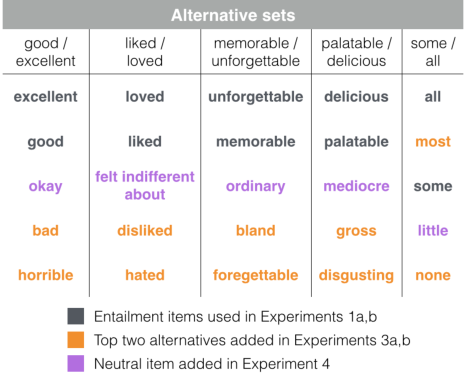
\includegraphics{figs/allScalesTable-1} \caption[Stimuli for Experiments 1a,b, 3a,b and 4]{Stimuli for Experiments 1a,b, 3a,b and 4.}\label{fig:allScalesTable}
\end{figure}
\end{CodeChunk}

\begin{CodeChunk}
\captionsetup{width=0.8\textwidth}\begin{figure*}[t]

{\centering 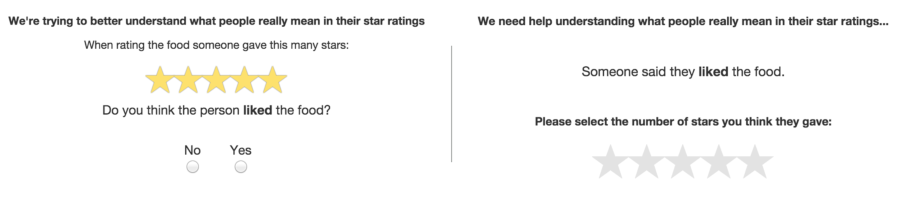
\includegraphics{figs/stimuli_exp1-1} 

}

\caption[(Left) A trial from Experiment 1a (literal listener) with the target scalar `liked]{(Left) A trial from Experiment 1a (literal listener) with the target scalar `liked.' (Right) A trial from Experiment 1b (pragmatic listener) with the target scalar `liked.'}\label{fig:stimuli_exp1}
\end{figure*}
\end{CodeChunk}

Experiment 1a and 1b were conducted to approximate literal listener
semantic distributions \(p_{L_0}(m \mid u)\) (Experiment 1a) and
pragmatic judgments \(p_{L_1}(m \mid u)\) (Experiment 1b) for five pairs
of scalar items taken from Tiel (2014). Scales and alternative
utterances are shown in Figure \ref{fig:allScalesTable}. Each pair of
scalar items consists of a ``weaker'' term (e.g. ``some'') and a
stronger term (e.g. ``all''). We begin with these classic members of the
Horn scale (Horn, 1972) as a test of the hypothesis that these
alternatives are all that is necessary to predict the strength of
listeners' pragmatic inferences.

\subsection{Methods}\label{methods}

\subsubsection{Participants}\label{participants}

We recruited 30 participants from Amazon Mechanical Turk (AMT) for
Experiment 1a; two participants were excluded because they reported
having a native language other than English for a final sample of 28
participants. We recruited 50 for Experiment 1b, also from AMT, and data
for 7 participants were excluded after participants either failed to
pass two training trials or reported a non-English native language,
leaving a total sample of 43 participants.

\subsubsection{Design and procedure}\label{design-and-procedure}

Figure \ref{fig:stimuli_exp1} shows the experimental setup for both
experiments. In Experiment 1a, the literal listener task, participants
were presented with a target scalar item and a star rating (1--5 stars)
and asked to judge the compatibility of the scalar item and star-rating.
Compatibility was assessed through a binary ``yes/no'' response to a
question of the form ``Do you think that the person thought the food was
\_\_\_\_?" where a target scalar was presented in the blank. Each
participant saw all scalar item and star rating combinations, in a
random oder.

In Experiment 1b, the pragmatic listener experiment, participants were
presented with a one-sentence prompt containing a target scalar item
such as ``Someone said they thought the food was \_\_\_\_\_.''
Participants were then asked to generate a star rating representing the
rating they thought the reviewer likely gave. Each participant was
presented with all scalar items in a random order.

\subsection{Results and Discussion}\label{results-and-discussion}

\begin{CodeChunk}
\captionsetup{width=0.8\textwidth}\begin{figure*}[t]

{\centering 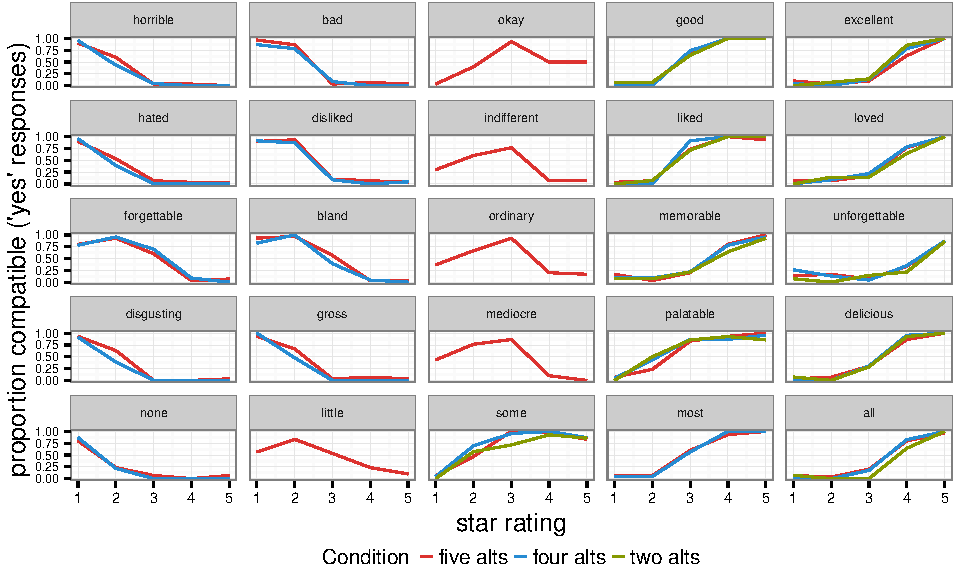
\includegraphics{figs/exp1Plots-1} 

}

\caption[Literal listener judgements from Experiments 1a, 3a, and 4]{Literal listener judgements from Experiments 1a, 3a, and 4. Proportion of participants indicating acceptability is shown on the vertical axis, with the horizontal axis showing number of stars on which the utterance was judged. Each line-type shows a different experiment, and colors indicate the different items in the scale (with the experiments including different numbers of items).  Each panel shows one scalar pair.}\label{fig:exp1Plots}
\end{figure*}
\end{CodeChunk}

Figure 2 plots literal listener \(p_{L0}(m|u)\) distributions obtained
in Experiments 1a, 3a and 4. Data from 1a is (\ldots{}). We see clear
variation in semantic judgments between scalar families in all
Experiments. For example, compatibility judgments for ``memorable'' and
``forgettable'' are more similar than those for ``good / excellent'' or
``liked / loved''. We will address distributional similarity across the
studies in later sections.

\section{Experiment 2: What are the
alternatives?}\label{experiment-2-what-are-the-alternatives}

In Experiment 1 we obtained literal semantic compatibility and pragmatic
judgments for five pairs of scalar terms. We would like to extend the
scale descriptions for each of these pairs to include other plausible
alternatives. We chose to take an empirical approach rather than assign
alternatives arbitrarily. We adopted a modified cloze task, inspired by
Experiment 2 in van Tiel (2014) and asked participants to generate
alternatives for us.

\subsection{Methods}\label{methods-1}

\subsubsection{Participants}\label{participants-1}

Using Amazon's Mechanical Turk, 30 workers were paid \$0.20 to
participate. All participants were native English speakers and naive to
the purpose of the experiment.

\subsubsection{Design and procedure}\label{design-and-procedure-1}

Participants were presented a target scalar term from our original
entailment set embedded in a sentence such as, ``In a recent restaurant
review someone said they thought they the food was \_\_\_\_" with a
target scalar presented in the ``\_\_\_\_." Participants were then asked
to generate plausible alternatives by responding to the question, ``If
they'd felt differently about the food, what other words could they have
used instead of \_\_\_\_\_?'' and asked to generate three unique
alternatives.

\subsection{Results and Discussion}\label{results-and-discussion-1}

Figure 3 plots the combined counts of alternatives generated for the
scalar items ``liked'' and ``loved.'' Alternative distributions for the
other scalar pairs (e.g.. ``good/excellent'',
``memorable/unforgettable'') were similarly long-tailed, however the
size and content of the alternate sets were diverse. (SOMETHING MORE
MORE FORMAL HERE???)

\begin{CodeChunk}
\captionsetup{width=0.8\textwidth}\begin{figure*}[t]

{\centering 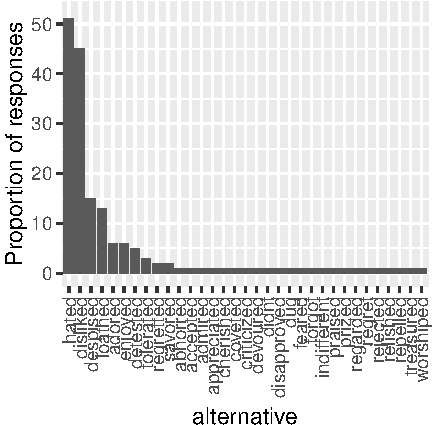
\includegraphics{figs/exp2_altsPlot_likedLoved-1} 

}

\caption[Caption goes here]{Caption goes here}\label{fig:exp2_altsPlot_likedLoved}
\end{figure*}
\end{CodeChunk}

\section{Experiment 3a,b: Incorporating top
alternatives}\label{experiment-3ab-incorporating-top-alternatives}

In Experiment 1a,b we measured literal semantics and pragmatic judgments
for Entailment scales. In Experiment 2, we asked participants to
generate plausible alternatives to these items. In Experiments 3a,b we
use the same experimental design for both literal semantics and
pragmatic judgment tasks, however we now expand the set of scalar items
to include the original Entailment pairs from Experiments 1a,b with the
top two alternatives generated for each scalar family by participants in
Experiment 2. The orange colored items in table 1 denote additional
scalar items added in Experiments 3a,b.

\subsection{Participants}\label{participants-2}

Participants for both studies were recruited on Amazon Mechanical Turk
and paid \$0.20 for their participation. Thirty participants were
recruited for Experiment 3a (Literal Listener task). Data for six
participants was thrown out after participants either failed to pass two
training trials or were not native English speakers, leaving a total
sample of 24 participants.

Fifty participants were recruited for Experiment 3b (Pragmatic Listener
task). Data for five participants was thrown out after participants
either failed to pass two training trials or were not native English
speakers, leaving a total sample of 45 participants.

\subsection{Procedure}\label{procedure}

The procedure of Experiments 3a,b follow the same form as Experiments
1a,b with the expanded set of target scalar items.

\subsection{Results and Discussion}\label{results-and-discussion-2}

Run glmer() here:

To test whether literal listener compatibility judgments differed
between Experiment 1a and 3a we ran a mixed effects model, regressing
responses to the binary compatibility measure on scale, degree, and
Experiment with random effects by subject. Results indicate (\ldots{})

Run elmer() here:

To test whether pragmatic judgments differed between Experiments 1b and
3b we ran a mixed effects model, regressing star-rating selections on
scale, scalar item and Experiment with random effects by subject.
Results indicate.

While conducting our analysis we realized that our literal semantic
distributions for each scalar family were roughly split between two
negative valenced items and two positively valenced items while neutral
alternatives appeared to be excluded. (This pattern was true of all the
scalar families, except for ``some ~all'' in which the top two
alternatives were positive valenced ``most'' and negative valenced
``none''.) In Experiment 4, we explore the addition of a neutrally
valenced scalar alternative for each scalar family.

\section{Experiment 4: Full scales - adding a neutral
alternative}\label{experiment-4-full-scales---adding-a-neutral-alternative}

In Experiment 4, we continue to extend the alternative sets, each by one
additional scalar item. While we simply took the top two alternatives
generated in Experiment 2 for the additional alternatives in Experiments
3a,b, in this case we chose a subjectively ``neutral'' valenced scalar
item from among the alternatives generated in Experiment 2. The idea was
to simulate a ``full'' set of alternatives, with negative, neutral and
positive valenced items for each scalar family. The purple colored items
in Table 1 denote additional scalar items added in Experiments 4.

\subsection{Participants}\label{participants-3}

Thirty participants were recruited on Amazon Mechanical Turk and paid
\$0.20 for their participation. There were no data exclusions due to
training failures or native language requirements, leaving a total
sample of thirty participants, all native English speakers, naive to the
purpose of the experiment.

\subsection{Procedure}\label{procedure-1}

The procedure of Experiment 4 follow the same form as Experiments 1a and
3a with the addition of a neutrally valence scalar item.

\subsection{Results and Discussion}\label{results-and-discussion-3}

Distributions for neutrally valenced scalar did appear fairly Gaussian,
occupying a literal semantic previously unoccupied by the other
alternatives.

Run glmer() here:

To test whether literal listener compatibility judgments differed
between Experiment 1a and 3a we ran a mixed effects model, regressing
responses to the binary compatibility measure on scale, degree, and
Experiment with random effects by subject. Results indicate (\ldots{})

Run elmer() here:

To test whether pragmatic judgments differed between Experiments 1b and
3b we ran a mixed effects model, regressing star-rating selections on
scale, scalar item and Experiment with random effects by subject.
Results indicate.

\section{Model Runs}\label{model-runs}

Using literal semantic data from Experiments 1a, 3a and 4 we conducted
three simulations with our model. Each simulation used the specific
literal semantic data to specify the scale representation available to
our model. The ``entailment'' model used only the original pair of
scalar items pulled from van Tiel (2014). These data were measured in
Experiment 1a. The ``Top two'' model extended the original set of
alternatives with the top two alternatives generated in Experiment 2.
These data were measured in Experiment 3a. The ``Full'' model included
the full set of alternatives, including a neutral valenced alternative.
These data were measured in Experiment 4.

\begin{CodeChunk}
\captionsetup{width=0.8\textwidth}\begin{figure*}[t]

{\centering 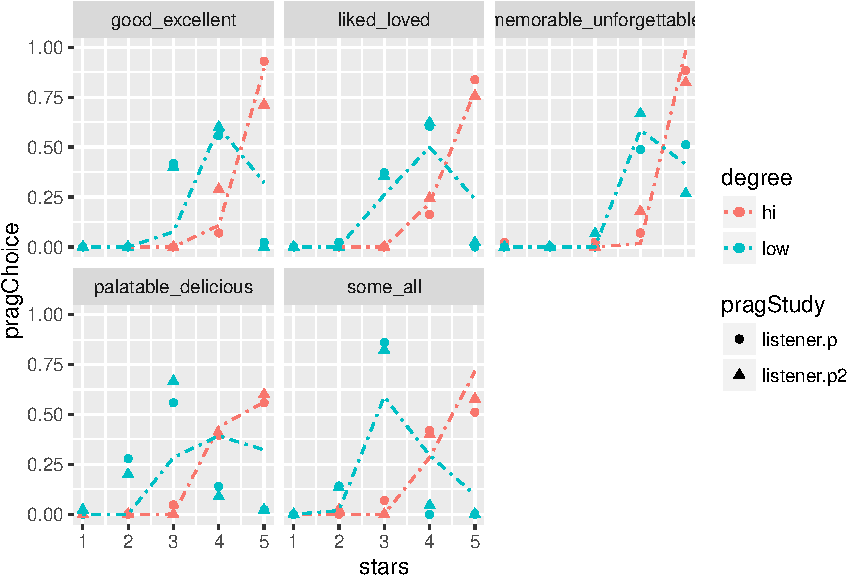
\includegraphics{figs/performancePlots-1} 

}

\caption[The left panel shows improved model fit as scale representations are enriched with more scalar items]{The left panel shows improved model fit as scale representations are enriched with more scalar items. Correlations are coputed using pragmatic judgment data from Experiments 1b and 3b. The right panel plots model predictions using full symmetric scales versus human judgments from Experiment 3b.}\label{fig:performancePlots}
\end{figure*}
\end{CodeChunk}

\section{General Discussion}\label{general-discussion}

By varying the type of scale representations available to our Bayesian
model we investigated the effects of alternatives on scalar implicature.
Model fit with human judgement was significantly improved by the
inclusion of alternatives beyond the typical ``strong'' and ``weak''
scalar items. In fact, we found that both neutral and negative valence
scalar items contribute to human-like implicature generation within our
framework.

\section{Acknowledgements}\label{acknowledgements}

Thanks to NSF BCS XYZ. Thanks to Michael Franke, Judith Degen, and Noah
Goodman.

\section{References}\label{references}

\setlength{\parindent}{-0.1in} \setlength{\leftskip}{0.125in} \noindent

Degen, J., \& Tanenhaus, M. K. (2015). Processing scalar implicature: A
constraint-based approach. \emph{Cognitive Science}, \emph{39}(4),
667--710.

Frank, M., \& Goodman, N. (2012). Predicting pragmatic reasoning in
language games. \emph{Science}, \emph{336}(6084), 998.

Franke, M. (2014). Typical use of quantifiers: A probabilistic speaker
model. In \emph{Proceedings of the 36th annual conference of the
cognitive science society} (pp. 487--492).

Goodman, N. D., \& Stuhlm{ü}ller, A. (2013). Knowledge and implicature:
Modeling language understanding as social cognition. \emph{Topics in
Cognitive Science}, \emph{5}(1), 173--184.

Grice, H. P. (1975). Logic and conversation. In P. Cole \& J. Morgan
(Eds.), \emph{Syntax and semantics} (Vol. 3). New York: Academic Press.

Horn, L. R. (1972). \emph{On the semantic properties of logical
operators.} (PhD thesis). University of California, Los Angeles.

Horn, L. R. (1984). Toward a new taxonomy for pragmatic inference:
Q-based and R-based implicature. \emph{Meaning, Form, and Use in
Context}, \emph{42}.

Levinson, S. C. (2000). \emph{Presumptive meanings: The theory of
generalized conversational implicature}. MIT Press.

Lewis, D. (1969). \emph{Convention: A philosophical study}. John Wiley
\& Sons.

Tiel, B. van. (2014). Quantity matters: Implicatures, typicality, and
truth.

Van Tiel, B., Van Miltenburg, E., Zevakhina, N., \& Geurts, B. (2014).
Scalar diversity. \emph{Journal of Semantics}, ffu017.

\end{document}
